\documentclass[12pt]{report}\usepackage[]{graphicx}\usepackage[]{color}
%% maxwidth is the original width if it is less than linewidth
%% otherwise use linewidth (to make sure the graphics do not exceed the margin)
\makeatletter
\def\maxwidth{ %
  \ifdim\Gin@nat@width>\linewidth
    \linewidth
  \else
    \Gin@nat@width
  \fi
}
\makeatother

\definecolor{fgcolor}{rgb}{0.345, 0.345, 0.345}
\newcommand{\hlnum}[1]{\textcolor[rgb]{0.686,0.059,0.569}{#1}}%
\newcommand{\hlstr}[1]{\textcolor[rgb]{0.192,0.494,0.8}{#1}}%
\newcommand{\hlcom}[1]{\textcolor[rgb]{0.678,0.584,0.686}{\textit{#1}}}%
\newcommand{\hlopt}[1]{\textcolor[rgb]{0,0,0}{#1}}%
\newcommand{\hlstd}[1]{\textcolor[rgb]{0.345,0.345,0.345}{#1}}%
\newcommand{\hlkwa}[1]{\textcolor[rgb]{0.161,0.373,0.58}{\textbf{#1}}}%
\newcommand{\hlkwb}[1]{\textcolor[rgb]{0.69,0.353,0.396}{#1}}%
\newcommand{\hlkwc}[1]{\textcolor[rgb]{0.333,0.667,0.333}{#1}}%
\newcommand{\hlkwd}[1]{\textcolor[rgb]{0.737,0.353,0.396}{\textbf{#1}}}%
\let\hlipl\hlkwb

\usepackage{framed}
\makeatletter
\newenvironment{kframe}{%
 \def\at@end@of@kframe{}%
 \ifinner\ifhmode%
  \def\at@end@of@kframe{\end{minipage}}%
  \begin{minipage}{\columnwidth}%
 \fi\fi%
 \def\FrameCommand##1{\hskip\@totalleftmargin \hskip-\fboxsep
 \colorbox{shadecolor}{##1}\hskip-\fboxsep
     % There is no \\@totalrightmargin, so:
     \hskip-\linewidth \hskip-\@totalleftmargin \hskip\columnwidth}%
 \MakeFramed {\advance\hsize-\width
   \@totalleftmargin\z@ \linewidth\hsize
   \@setminipage}}%
 {\par\unskip\endMakeFramed%
 \at@end@of@kframe}
\makeatother

\definecolor{shadecolor}{rgb}{.97, .97, .97}
\definecolor{messagecolor}{rgb}{0, 0, 0}
\definecolor{warningcolor}{rgb}{1, 0, 1}
\definecolor{errorcolor}{rgb}{1, 0, 0}
\newenvironment{knitrout}{}{} % an empty environment to be redefined in TeX

\usepackage{alltt}

%%%%%%%%%%%%%%%%%%%%%%
%%%% conditionals %%%%
%%%%%%%%%%%%%%%%%%%%%%
\newif\ifanswer
\answertrue %% comment out to hide answers
%%%%==============%%%%

%%%%%%%%%%%%%%%%%
%%%% read me %%%%
%%%%%%%%%%%%%%%%%
% 1. When open a device tikz(), an absolute file path should be like
% tikz(file="C:/Users/leejung.MED/Dropbox/Avril_book/aat_est.tex", width=5, height=5)
%
% 2.
%
%%%%=========%%%%

%%%%%%%%%%%%%%%%%%%%%%%%%%%%%
%%%% packages are loaded %%%%
%%%%%%%%%%%%%%%%%%%%%%%%%%%%%
\usepackage[hangul]{kotex} %% for Korean. Use \usepackage[hangul]{kotex} for FULL korean environment
\usepackage{bm} %% Needed for bold italic in math mode
\usepackage{tikz} %% for tikzDevice and tikzpicture
\usepackage{pgfplots} %% Needed for TikZ
\usetikzlibrary{arrows} %% Needed for tikz axis arrow shape
\usepackage{tkz-base} %% Needed for creating 2d figures
\usepackage{tkz-euclide} %% Needed for creating 2d figures
\usetkzobj{all} %% Needed for creating 2d figures
\usepackage{amssymb} %% some symbols like \square
%%%%=====================%%%%

%%%%%%%%%%%%%%%%%%%%%%%%%%%%
%%%% colors are defined %%%%
%%%%%%%%%%%%%%%%%%%%%%%%%%%%
\def\red{\textcolor{red}}
\def\green{\textcolor{green}}
\def\blue{\textcolor{blue}}
\def\yellow{\textcolor{yellow}}
%%%%====================%%%%

%%%%%%%%%%%%%%%%%%%%%%%%%%%%%%%%%%%
%%%% load "tikzDevice" package %%%%
%%%%%%%%%%%%%%%%%%%%%%%%%%%%%%%%%%%
%<<echo=FALSE, warning=FALSE>>=
%library(tikzDevice)
%@
%%%%===========================%%%%
\IfFileExists{upquote.sty}{\usepackage{upquote}}{}
\begin{document}

\begin{enumerate}
\item 정사각형 $\square ABCD$의 변 $\overline{AB}$와 $\overline{AD}$ 위에 $\angle CPB=60^\circ$, $\angle QCP=45^\circ$가 되도록 점 $P$, $Q$를 잡을 때 $\angle QPC$를 구하여라.

\begin{center}
\begin{tikzpicture}[scale=1]
  \tkzDefPoint(0,0){A} \tkzLabelPoint[below left](A){$A$}
  \tkzDefPoint(6,0){B} \tkzLabelPoint[below right](B){$B$}
  \tkzDefPoint(6,6){C} \tkzLabelPoint[above right](C){$C$}
  \tkzDefPoint(0,6){D} \tkzLabelPoint[above left](D){$D$}
  \tkzDrawPolygon(A,B,C,D)
  
  % lower side
  \tkzDefShiftPoint[C](240:2){PP}
  \tkzInterLL(C,PP)(A,B) \tkzGetPoint{P}
  \tkzLabelPoint[below](P){$P$}
  
  % left side
  \tkzDefShiftPoint[C](195:1){QQ}
  \tkzInterLL(C,QQ)(A,D) \tkzGetPoint{Q}
  \tkzLabelPoint[left](Q){$Q$}
  
  \tkzDrawPolygon(P,C,Q)
  \tkzMarkRightAngles(A,B,C C,D,A D,A,B)
  \tkzMarkSegments[mark=||, size=5](A,B B,C C,D D,A)
  \tkzMarkAngle[size=0.5](C,P,Q) 
  \tkzLabelAngle(C,P,Q){$x$}
  \tkzMarkAngle[size=0.5](Q,C,P)
  \tkzLabelAngle(Q,C,P){$45^{\circ}$}
  \tkzMarkAngle[size=0.6](B,P,C)
  \tkzLabelAngle(B,P,C){$60^{\circ}$}
\end{tikzpicture}
\end{center}

\ifanswer
\textbf{$\langle$풀이$\rangle$}
\begin{center}
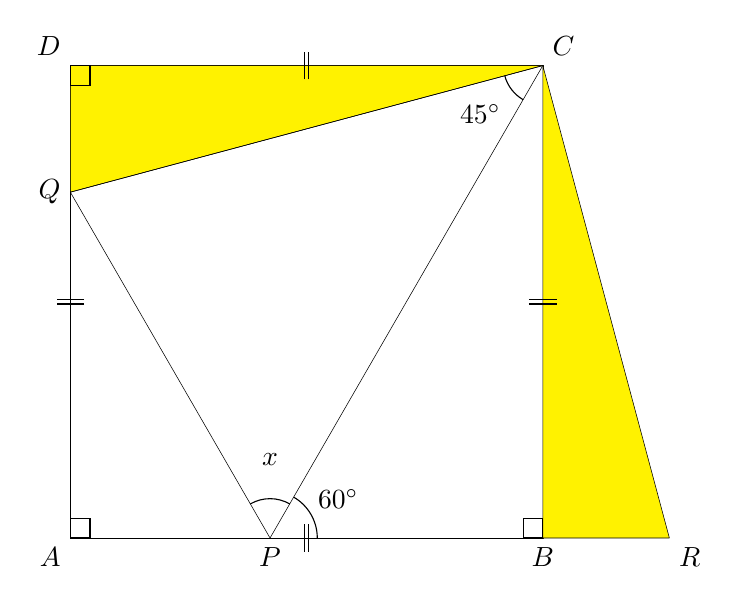
\begin{tikzpicture}[scale=1]
  \tkzDefPoint(0,0){A} \tkzLabelPoint[below left](A){$A$}
  \tkzDefPoint(6,0){B} \tkzLabelPoint[below](B){$B$}
  \tkzDefPoint(6,6){C} \tkzLabelPoint[above right](C){$C$}
  \tkzDefPoint(0,6){D} \tkzLabelPoint[above left](D){$D$}
  \tkzDrawPolygon(A,B,C,D)
  
  % lower side
  \tkzDefShiftPoint[C](240:2){PP}
  \tkzInterLL(C,PP)(A,B) \tkzGetPoint{P}
  \tkzLabelPoint[below](P){$P$}
  
  % left side
  \tkzDefShiftPoint[C](195:1){QQ}
  \tkzInterLL(C,QQ)(A,D) \tkzGetPoint{Q}
  \tkzLabelPoint[left](Q){$Q$}
  
  % copy
  \tkzDefShiftPoint[C](285:1){RR}
  \tkzInterLL(C,RR)(A,B) \tkzGetPoint{R}
  \tkzLabelPoint[below right](R){$R$}
  
  \tkzDrawPolygon[fill=yellow](C,D,Q)
  \tkzDrawPolygon[fill=yellow](C,B,R)
  
  \tkzDrawPolygon(P,C,Q)
  \tkzMarkRightAngles(A,B,C C,D,A D,A,B)
  \tkzMarkSegments[mark=||, size=5](A,B B,C C,D D,A)
  \tkzMarkAngle[size=0.5](C,P,Q) 
  \tkzLabelAngle(C,P,Q){$x$}
  \tkzMarkAngle[size=0.5](Q,C,P)
  \tkzLabelAngle(Q,C,P){$45^{\circ}$}
  \tkzMarkAngle[size=0.6](B,P,C)
  \tkzLabelAngle(B,P,C){$60^{\circ}$}
  
  
\end{tikzpicture}
\end{center}
그림에서 $\triangle CDQ$와 $\triangle CBR$이 합동이 되도록 점 $R$을 잡으면 $\triangle CPQ$와 $\triangle CPR$이 합동이 되므로 $x=60^\circ$가 된다.
\fi

\newpage

\item 다음 그림에서 $\angle ABC=100^\circ$이고 $\overline{AB}=\overline{BC}$, $\overline{BD}=\overline{AC}$일 때 $\angle ACD$를 구하여라 

\begin{center}
\begin{tikzpicture}[scale=1]
  \tkzDefPoint(0,0){A} \tkzLabelPoint[above left](A){$A$}
  \tkzDefShiftPoint[A](40:5){B} \tkzLabelPoint[above](B){$B$}
  \tkzDefShiftPoint[B](320:5){C} \tkzLabelPoint[right](C){$C$}
  \tkzDrawPolygon(A,B,C)
  
  \tkzDefShiftPoint[C](190:1){DD}
  \tkzInterLL(C,DD)(B,A) \tkzGetPoint{D} 
  \tkzLabelPoint[left](D){$D$}
  \tkzDrawPolygon(A,D,C)
  
  \tkzMarkAngle[size=0.5](A,B,C)
  \tkzLabelAngle(A,B,C){$100^\circ$}
  \tkzMarkSegments[mark=||, size=5](A,B B,C)
  \tkzMarkSegments[mark=|, size=5](D,B A,C)
  
  \tkzMarkAngle[size=1.5](A,C,D)
  \tkzLabelAngle[pos=-1.8](A,C,D){$x$}
   
\end{tikzpicture}
\end{center}

\ifanswer
\textbf{$\langle$풀이$\rangle$}
\begin{center}
\begin{tikzpicture}[scale=1]

  \tkzDefPoint(0,0){A} \tkzLabelPoint[above left](A){$A$}
  \tkzDefShiftPoint[A](40:5){B} \tkzLabelPoint[above](B){$B$}
  \tkzDefShiftPoint[B](320:5){C} \tkzLabelPoint[right](C){$C$}
  \tkzDrawPolygon(A,B,C)
  
  \tkzDefShiftPoint[C](190:1){DD}
  \tkzInterLL(C,DD)(B,A) \tkzGetPoint{D} 
  \tkzLabelPoint[left](D){$D$}
  \tkzDrawPolygon(A,D,C)
  
  \tkzMarkAngle[size=0.5](A,B,C)
  \tkzMarkSegments[mark=||, size=5](A,B B,C)
  \tkzMarkSegments[mark=|, size=5](D,B A,C)
  
  \tkzMarkAngle[size=0.5](B,C,A)
  \tkzLabelAngle(B,C,A){$40^\circ$}
  
  \tkzMarkAngle[size=1.5](A,C,D)
  \tkzLabelAngle[pos=-1.8](A,C,D){$x$}
  
  \tkzDefShiftPoint[D](0:1){EE}
  \tkzDefShiftPoint[B](260:1){FF}
  \tkzInterLL(D,EE)(B,FF) \tkzGetPoint{E}
  \tkzLabelPoint[below right](E){$E$}
  
  \tkzDrawSegments(D,E B,E E,C)
  \tkzMarkSegments[mark=||, size=5](D,E B,E E,C)
  
  \tkzLabelAngle(A,B,E){$40^\circ$}
  \tkzLabelAngle(E,B,C){$60^\circ$}
  

\end{tikzpicture}
\end{center}
$\overline{BE}=\overline{DE}$가 되도록 점 $E$를 잡으면 $\triangle EBD$와 $\triangle BAC$는 합동이다. 따라서 $\triangle BEC$는 정삼각형이 되고 $\triangle ECD$는 이등변삼각형이 된다. $\angle DEC=160^\circ$이므로 $\angle ECD=10^\circ$, 따라서 $x=10^\circ$. 
\fi

\newpage

\item $\triangle ABC$의 변 $\overline{AB}$, $\overline{BC}$ 위에 각각 점 $D$, $E$를 $\overline{AD}=\overline{DE}=\overline{EC}$가 되도록 잡았을 때 $\angle BCA$를 구하여라. 단 $\angle ABC=60^\circ$이고 $\angle BED=90^\circ$이다.

\begin{center}
\begin{tikzpicture}[scale=1]

  \tkzDefPoint(0,0){A} \tkzLabelPoint[left](A){$A$}
  \tkzDefShiftPoint[A](45:7){B}
  \tkzLabelPoint[above](B){$B$}
  \tkzDefShiftPoint[B](-75:1){CC}
  \tkzDefShiftPoint[A](0:1){DD}
  \tkzInterLL(A,DD)(B,CC) \tkzGetPoint{C}
  \tkzLabelPoint[right](C){$C$}
  
  \tkzDefShiftPoint[A](-15:1){PP}
  \tkzDefShiftPoint[C](195:1){QQ}
  \tkzInterLL(A,PP)(C,QQ) \tkzGetPoint{P}
  %\tkzDrawSegment(A,P)
  
  \tkzDefShiftPoint[P](105:1){RR}
  \tkzInterLL(P,RR)(A,B) \tkzGetPoint{D}
  \tkzLabelPoint[above left](D){$D$}
  %\tkzDrawSegment(Q,P)
  
  \tkzDefShiftPoint[D](15:1){SS}
  \tkzInterLL(D,SS)(C,B) \tkzGetPoint{E}
  \tkzDrawSegment(D,E)
  \tkzLabelPoint[right](E){$E$}
  
  \tkzMarkSegments[mark=||, size=5](A,D D,E E,C)
  
  \tkzDrawPolygon(A,B,C)
  \tkzMarkAngle[size=0.5](D,B,E)
  \tkzLabelAngle(D,B,E){$60^\circ$}
  
  \tkzMarkAngle[size=0.5](B,C,A)
  \tkzLabelAngle(B,C,A){$x$}
  
  \tkzMarkRightAngle(B,E,D)
  
  
\end{tikzpicture}
\end{center}

\ifanswer
\textbf{$\langle$풀이$\rangle$}
\begin{center}
\begin{tikzpicture}[scale=1]

  \tkzDefPoint(0,0){A} \tkzLabelPoint[left](A){$A$}
  \tkzDefShiftPoint[A](45:7){B}
  \tkzLabelPoint[above](B){$B$}
  \tkzDefShiftPoint[B](-75:1){CC}
  \tkzDefShiftPoint[A](0:1){DD}
  \tkzInterLL(A,DD)(B,CC) \tkzGetPoint{C}
  \tkzLabelPoint[right](C){$C$}
  
  \tkzDefShiftPoint[A](-15:1){PP}
  \tkzDefShiftPoint[C](195:1){QQ}
  \tkzInterLL(A,PP)(C,QQ) \tkzGetPoint{P}
  %\tkzDrawSegment(A,P)
  
  \tkzDefShiftPoint[P](105:1){RR}
  \tkzInterLL(P,RR)(A,B) \tkzGetPoint{D}
  \tkzLabelPoint[above left](D){$D$}
  %\tkzDrawSegment(Q,P)
  
  \tkzDefShiftPoint[D](15:1){SS}
  \tkzInterLL(D,SS)(C,B) \tkzGetPoint{E}
  \tkzDrawSegment(D,E)
  \tkzLabelPoint[right](E){$E$}
  
  \tkzMarkSegments[mark=||, size=5](A,D D,E E,C)
  
  \tkzDrawPolygon(A,B,C)
  \tkzMarkAngle[size=0.5](D,B,E)
  \tkzLabelAngle(D,B,E){$60^\circ$}
  
  \tkzMarkAngle[size=0.5](B,C,A)
  \tkzLabelAngle(B,C,A){$x$}
  
  \tkzMarkRightAngle(B,E,D)
  
  \tkzDefShiftPoint[D](-75:1){FF}
  \tkzDefShiftPoint[A](-15:1){GG}
  \tkzInterLL(D,FF)(A,GG) \tkzGetPoint{F}
  \tkzLabelPoint[below](F){$F$}
  \tkzDrawSegments(A,F D,F F,C)
  \tkzMarkSegments[mark=||, size=5](A,F D,F F,C)
   
\end{tikzpicture}
\end{center}
$\overline{AD}=\overline{DF}=\overline{AF}$가 되도록 점 $F$를 잡으면 $\square DECF$는 정사각형이 되므로 $\triangle AFC$는 $\angle AFC=150^\circ$인 이등변 삼각형이다. 따라서 $x=90^\circ-15^\circ=75^\circ$. 

\fi

\newpage

\item 그림과 같이 $\angle B=20^\circ$ 인 이등변 삼각형 $\triangle ABC$의 변 $\overline{AB}$, $\overline{CB}$위에 각각 점 $E$, $D$를 $\angle ECA=50^\circ$, $\angle DAC=60^\circ$가 되도록 잡았을 때 $\angle EDA$를 구하여라.

\begin{center}
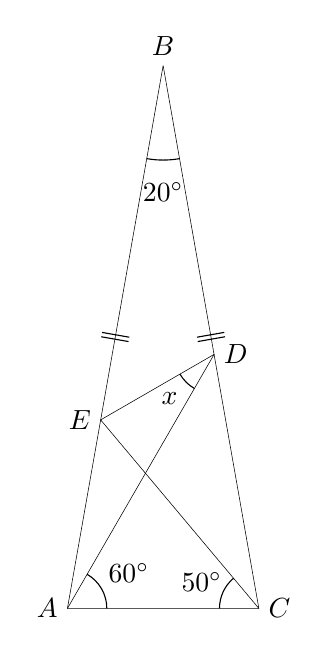
\begin{tikzpicture}

  \tkzDefPoint(0,0){A} \tkzLabelPoint[left](A){$A$}
  \tkzDefShiftPoint[A](80:7){B} \tkzLabelPoint[above](B){$B$}
  \tkzDefShiftPoint[B](-80:7){C} \tkzLabelPoint[right](C){$C$}
  \tkzDrawPolygon(A,B,C)
  \tkzMarkSegments[mark=||, size=5](A,B B,C)
  
  \tkzDefShiftPoint[A](60:1){DD}
  \tkzInterLL(A,DD)(B,C) \tkzGetPoint{D} 
  \tkzLabelPoint[right](D){$D$}
  \tkzDrawSegment(A,D)
  
  \tkzDefShiftPoint[C](130:1){EE}
  \tkzInterLL(C,EE)(A,B) \tkzGetPoint{E} 
  \tkzLabelPoint[left](E){$E$}
  \tkzDrawSegment(C,E)
  \tkzDrawSegment(E,D)
  
  \tkzMarkAngle[size=1.2](A,B,C)
  \tkzLabelAngle[pos=1.6](A,B,C){$20^\circ$}
  
  \tkzMarkAngle[size=0.5](C,A,D)
  \tkzLabelAngle[pos=0.9](C,A,D){$60^\circ$}
  
  \tkzMarkAngle[size=0.5](E,C,A)
  \tkzLabelAngle[pos=0.8](E,C,A){$50^\circ$}
  
  \tkzMarkAngle[size=0.5](E,D,A)
  \tkzLabelAngle[pos=0.8](E,D,A){$x$}
  
\end{tikzpicture}
\end{center}

\ifanswer
\textbf{$\langle$풀이$\rangle$}
\begin{center}
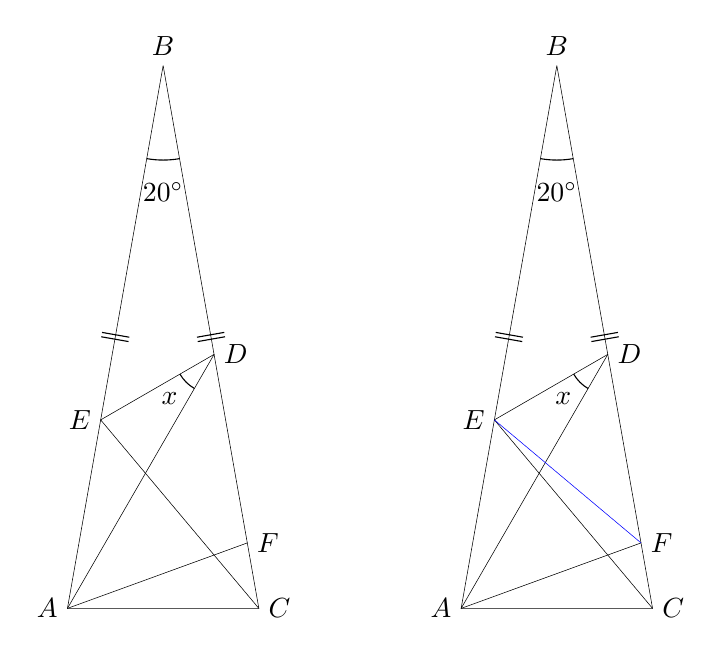
\begin{tikzpicture}

  \tkzDefPoint(0,0){A} \tkzLabelPoint[left](A){$A$}
  \tkzDefShiftPoint[A](80:7){B} \tkzLabelPoint[above](B){$B$}
  \tkzDefShiftPoint[B](-80:7){C} \tkzLabelPoint[right](C){$C$}
  \tkzDrawPolygon(A,B,C)
  \tkzMarkSegments[mark=||, size=5](A,B B,C)
  
  \tkzDefShiftPoint[A](60:1){DD}
  \tkzInterLL(A,DD)(B,C) \tkzGetPoint{D} 
  \tkzLabelPoint[right](D){$D$}
  \tkzDrawSegment(A,D)
  
  \tkzDefShiftPoint[C](130:1){EE}
  \tkzInterLL(C,EE)(A,B) \tkzGetPoint{E} 
  \tkzLabelPoint[left](E){$E$}
  \tkzDrawSegment(C,E)
  \tkzDrawSegment(E,D)
  
  \tkzMarkAngle[size=1.2](A,B,C)
  \tkzLabelAngle[pos=1.6](A,B,C){$20^\circ$}
  
  %\tkzMarkAngle[size=0.5](C,A,D)
  %\tkzLabelAngle[pos=0.9](C,A,D){$60^\circ$}
  
  %\tkzMarkAngle[size=0.5](E,C,A)
  %\tkzLabelAngle[pos=0.8](E,C,A){$50^\circ$}
  
  \tkzMarkAngle[size=0.5](E,D,A)
  \tkzLabelAngle[pos=0.8](E,D,A){$x$}
  \tkzDefShiftPoint[A](20:1){FF}
  \tkzInterLL(A,FF)(B,C) \tkzGetPoint{F} 
  \tkzLabelPoint[right](F){$F$}
  \tkzDrawSegments(A,F)

\begin{scope}[xshift=5cm]

  \tkzDefPoint(0,0){A} \tkzLabelPoint[left](A){$A$}
  \tkzDefShiftPoint[A](80:7){B} \tkzLabelPoint[above](B){$B$}
  \tkzDefShiftPoint[B](-80:7){C} \tkzLabelPoint[right](C){$C$}
  \tkzDrawPolygon(A,B,C)
  \tkzMarkSegments[mark=||, size=5](A,B B,C)
  
  \tkzDefShiftPoint[A](60:1){DD}
  \tkzInterLL(A,DD)(B,C) \tkzGetPoint{D} 
  \tkzLabelPoint[right](D){$D$}
  \tkzDrawSegment(A,D)
  
  \tkzDefShiftPoint[C](130:1){EE}
  \tkzInterLL(C,EE)(A,B) \tkzGetPoint{E} 
  \tkzLabelPoint[left](E){$E$}
  \tkzDrawSegment(C,E)
  \tkzDrawSegment(E,D)
  
  \tkzMarkAngle[size=1.2](A,B,C)
  \tkzLabelAngle[pos=1.6](A,B,C){$20^\circ$}
  
  %\tkzMarkAngle[size=0.5](C,A,D)
  %\tkzLabelAngle[pos=0.9](C,A,D){$60^\circ$}
  
  %\tkzMarkAngle[size=0.5](E,C,A)
  %\tkzLabelAngle[pos=0.8](E,C,A){$50^\circ$}
  
  \tkzMarkAngle[size=0.5](E,D,A)
  \tkzLabelAngle[pos=0.8](E,D,A){$x$}
  \tkzDefShiftPoint[A](20:1){FF}
  \tkzInterLL(A,FF)(B,C) \tkzGetPoint{F} 
  \tkzLabelPoint[right](F){$F$}
  \tkzDrawSegments(A,F)
  \tkzDrawSegments[color=blue](E,F)

\end{scope}
\end{tikzpicture} 
\end{center}
\fi
$\angle AFC=80^\circ$가 되도록 점 $F$를 변 $\overline{BC}$위에 잡으면 $\triangle AEC$와 $\triangle AFC$는 각각 이등변 삼각형이 되므로 $\overline{AE}=\overline{AF}$. $\angle EAF=60^\circ$이므로 $\triangle AEF$는 정삼각형이고 따라서 $\overline{EF}=\overline{AF}$. 또한 $\angle FAD=\angle FDA=40^\circ$ 이므로 $\triangle FAD$는 이등변 삼각형이고 특히 $\overline{AF}=\overline{DF}$. 이제  $\angle EFD=40^\circ$이고 $\triangle EFD$ 또한 이등변 삼각형이므로 $x=30^\circ$.  

\end{enumerate}
\end{document}


